\chapter{The main window}\label{ch:window}

\begin{figure}[H]
  \centering
  \begin{tikzpicture}
    \node[anchor=south west, inner sep=0] (img)
      {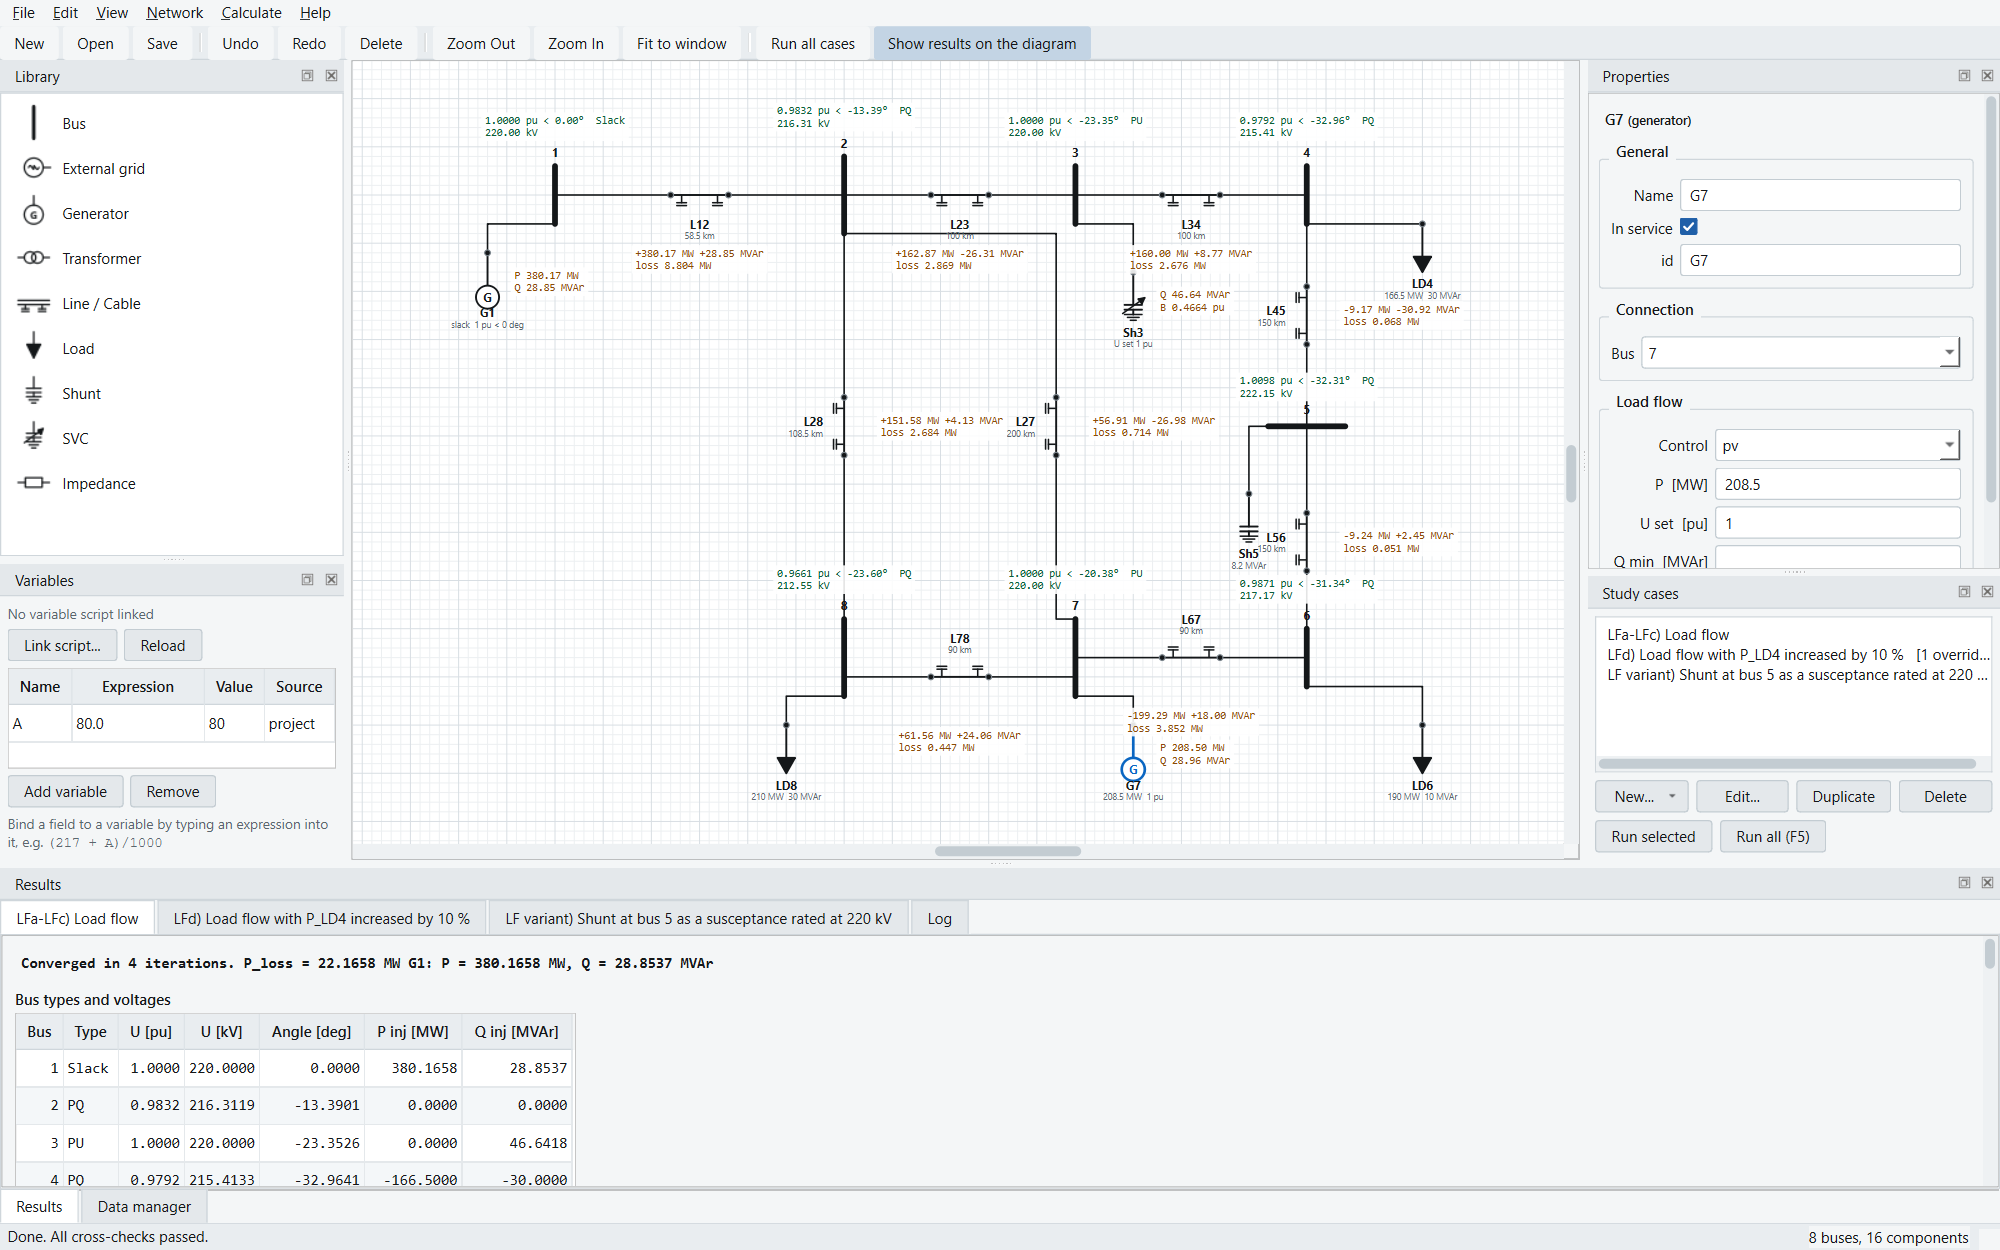
\includegraphics[width=\linewidth]{figures/window-overview.png}};
    \begin{scope}[x={(img.south east)}, y={(img.north west)}]
      % Generated by tools/make_manual.py: callout positions on window-overview.png.
\windowcallout{0.3300}{0.9900}{1}% menubar
\windowcallout{0.6200}{0.9650}{2}% toolbar
\windowcallout{0.1066}{0.9400}{3}% library
\windowcallout{0.1066}{0.5370}{4}% variables
\windowcallout{0.2002}{0.9300}{5}% canvas
\windowcallout{0.9072}{0.9400}{6}% properties
\windowcallout{0.9072}{0.5270}{7}% cases
\windowcallout{0.2000}{0.2940}{8}% results
\windowcallout{0.5000}{0.0120}{9}% status

    \end{scope}
  \end{tikzpicture}
  \caption{The main window with the load flow example after \keys{F5}. The numbers
    match the list below.}\label{fig:window}
\end{figure}

\begin{enumerate}[label=\calloutnum{\arabic*}, leftmargin=2.2em]
  \item \textbf{Menu bar}: \gui{File}, \gui{Edit}, \gui{View}, \gui{Network},
    \gui{Calculate} and \gui{Help} (\cref{sec:menus}).
  \item \textbf{Toolbar}: the most used commands (\cref{sec:toolbar}).
  \item \textbf{Library}: the component palette. Click an entry and then the canvas to
    place it, or drag it onto the canvas (\cref{sec:placing}).
  \item \textbf{Variables}: the project variables, and those read from a linked script
    (\cref{ch:parameters}).
  \item \textbf{Canvas}: the single-line diagram. With results shown, it carries their
    annotations (\cref{sec:annotations}).
  \item \textbf{Properties}: a form for the selected element or elements, generated from
    their fields (\cref{sec:properties}).
  \item \textbf{Study cases}: the cases \keys{F5} runs, with buttons to create, edit,
    duplicate, delete and run them (\cref{ch:cases}).
  \item \textbf{Results} and \textbf{Data manager}: two tabs of one panel. The first holds
    a tab per study result plus a \gui{Log} (\cref{ch:results}), the second the component
    tables (\cref{ch:data-manager}).
  \item \textbf{Status bar}: messages on the left, and the number of buses and components
    on the right.
\end{enumerate}

The panels are dock widgets. Drag a panel by its title bar to move it, to stack it with
another panel as a tab, or to float it as a separate window. Close one with the
\gui{\texttimes} button on its title bar, and bring it back from the \gui{View} menu.
\app\ remembers the layout and the window size between sessions. A layout saved by an
older version that lacked one of today's panels is ignored, and the default layout comes
back.

\section{Menus}\label{sec:menus}

\subsection{File}

\begin{reftable}{@{}>{\raggedright\arraybackslash}p{4.3cm}>{\raggedright\arraybackslash}p{2.6cm}X@{}}
\toprule
\sffamily\bfseries Entry & \sffamily\bfseries Shortcut & \sffamily\bfseries What it does \\ \midrule
\gui{New} & \keys{\ctrl + N} & An empty project. Asks first if the current one has unsaved changes. \\
\gui{Open...} & \keys{\ctrl + O} & Open a \file{.psn} project. \\
\gui{Open recent} & & The last projects opened. \\
\gui{Load Assignment S1 example} & & The S1 network as an untitled copy. \\
\gui{Save} & \keys{\ctrl + S} & Save the project; an untitled one asks for a name. \\
\gui{Save As...} & \keys{\ctrl + \shift + S} & Save under another name. \\
\gui{Export results...} & \keys{\ctrl + E} & Write the last run's results as text, CSV, LaTeX or JSON (\cref{sec:export-results}). \\
\gui{Export diagram...} & \keys{\ctrl + \shift + E} & Save the diagram as PNG, SVG or PDF (\cref{sec:export-diagram}). \\
\gui{Exit} & \keys{\ctrl + Q} & Close \app; asks to save unsaved changes. \\
\bottomrule
\end{reftable}

\subsection{Edit}

\begin{reftable}{@{}>{\raggedright\arraybackslash}p{4.3cm}>{\raggedright\arraybackslash}p{2.6cm}X@{}}
\toprule
\sffamily\bfseries Entry & \sffamily\bfseries Shortcut & \sffamily\bfseries What it does \\ \midrule
\gui{Undo}, \gui{Redo} & \keys{\ctrl + Z}, \keys{\ctrl + Y} & Undo or redo the last change; the entry names it. \\
\gui{Cut}, \gui{Copy}, \gui{Paste} & \keys{\ctrl + X}, \keys{\ctrl + C}, \keys{\ctrl + V} & The clipboard, for elements on the canvas (\cref{sec:clipboard}). \\
\gui{Duplicate} & \keys{\ctrl + D} & Copy and paste the selection in one step. \\
\gui{Delete} & \keys{Del} & Delete the selection (\cref{sec:deleting}). \\
\gui{Select All} & \keys{\ctrl + A} & Select every element. \\
\gui{Find element...} & \keys{\ctrl + F} & Select an element by name or id and centre the diagram on it (\cref{sec:find}). \\
\gui{Rotate 90 deg} & \keys{\ctrl + \Alt + R} & Rotate the selected symbols. \\
\gui{Flip bus orientation} & \keys{\ctrl + \Alt + O} & Switch the selected buses between vertical and horizontal. \\
\bottomrule
\end{reftable}

The clipboard shortcuts act on the canvas only when it has the keyboard focus, so that
\keys{\ctrl + C} in a result table copies the table and \keys{\ctrl + V} in a field pastes
text.

\subsection{View}

\begin{reftable}{@{}>{\raggedright\arraybackslash}p{4.3cm}>{\raggedright\arraybackslash}p{2.6cm}X@{}}
\toprule
\sffamily\bfseries Entry & \sffamily\bfseries Shortcut & \sffamily\bfseries What it does \\ \midrule
\gui{Zoom In}, \gui{Zoom Out} & \keys{\ctrl + +}, \keys{\ctrl + -} & Zoom the canvas. \keys{\ctrl} + mouse wheel zooms around the cursor. \\
\gui{Fit to window} & \keys{\ctrl + 0} & Show the whole diagram. \\
\gui{Actual size} & \keys{\ctrl + 1} & One scene unit per pixel. \\
\gui{Show results on the diagram} & \keys{\ctrl + R} & Show or hide the annotations of the selected result (\cref{sec:annotations}). \\
\gui{Colour by} & & \gui{Nothing}, \gui{Voltage level} or \gui{Voltage result} (\cref{sec:colouring}). \\
\gui{Library} \dots\ \gui{Results} & & Show or hide each panel. \\
\gui{Data manager} & \keys{\ctrl + \shift + D} & Bring the data manager forward, on the type of the selected element. \\
\bottomrule
\end{reftable}

\subsection{Network}

\gui{Base settings...} sets the base power, the frequency, the base reference bus and its
base voltage (\cref{ch:bases}).

\subsection{Calculate}

\begin{minipage}[t]{0.62\linewidth}
\gui{Run all cases} (\keys{F5}) runs every study case of the project. A project without
cases runs every study once, with its default options. Below it is one submenu per study
group: \gui{Model} (per-unit model, admittance matrix, sequence model), \gui{Assignment
S1} (S1a--S1c) and \gui{Network} (linear voltages, Thevenin equivalent, short circuit, load
flow, unbalanced load).

Choosing a study from these submenus opens the dialog of the study's \emph{own case},
whose id is the study's key. Accept it and the case is saved in the project and run.
\Cref{sec:own-case} explains this in detail.
\end{minipage}\hfill
\begin{minipage}[t]{0.33\linewidth}\vspace{0pt}
  \centering\shot[0.95\linewidth]{menu-calculate.png}
\end{minipage}

\subsection{Help}

\gui{About PowerLab} shows the version and what the program does.

\section{The toolbar}\label{sec:toolbar}

From left to right: \gui{New}, \gui{Open}, \gui{Save}; \gui{Undo}, \gui{Redo},
\gui{Delete}; \gui{Zoom Out}, \gui{Zoom In}, \gui{Fit to window}; \gui{Run all cases};
and \gui{Show results on the diagram}, a toggle for the annotations. The buttons do the
same as the menu entries of the same name.

\section{When results go stale}

Any change to the electrical model makes the results on screen out of date: a field, a
connection, an element added, deleted or taken out of service, a variable, the bases.
Moving symbols, editing wire bends and dragging labels change only the drawing, so they
leave the results alone. \app\ shows stale results in three ways:

\begin{itemize}
  \item the result tabs get an asterisk (\gui{LFa-LFc) Load flow *});
  \item a banner over the canvas reads \emph{``The model has changed, so the results below
    are out of date. Press F5 to run the studies again.''};
  \item the diagram annotations are removed, because they no longer describe the network
    drawn.
\end{itemize}

The tables stay readable, so you can compare before and after. Run the cases again to
bring everything up to date.
